%%Copyright 2021. Any replication of this document is permissible. The primary package of this document is from cjquines%%

%%PRIMARY PREAMBLE%%
\documentclass[10pt,paper=letter]{scrartcl}
\usepackage[boxthm, alttitle]{cjquines}
\usepackage{jrobaob}
\usepackage{enumitem}
\usepackage[makeroom]{cancel}
\usepackage{incgraph,tikz}

\begin{document}

\incgraph[documentpaper,
  overlay={\node[red] at (page.center) {\Huge };}]
  [width=\paperwidth,height=\paperheight]{cOVERPAGE.png}

\newpage

\title{Basic Calculus Reviewer}
\subtitle{Ateneo De Davao University Senior High School}
\author{Josh Robert Obaob}
\date{March 3, 2022} 

\maketitle
\setlength{\unitlength}{1in}
\begin{picture}(0,0)
  \put(5.5,0.5){\hbox{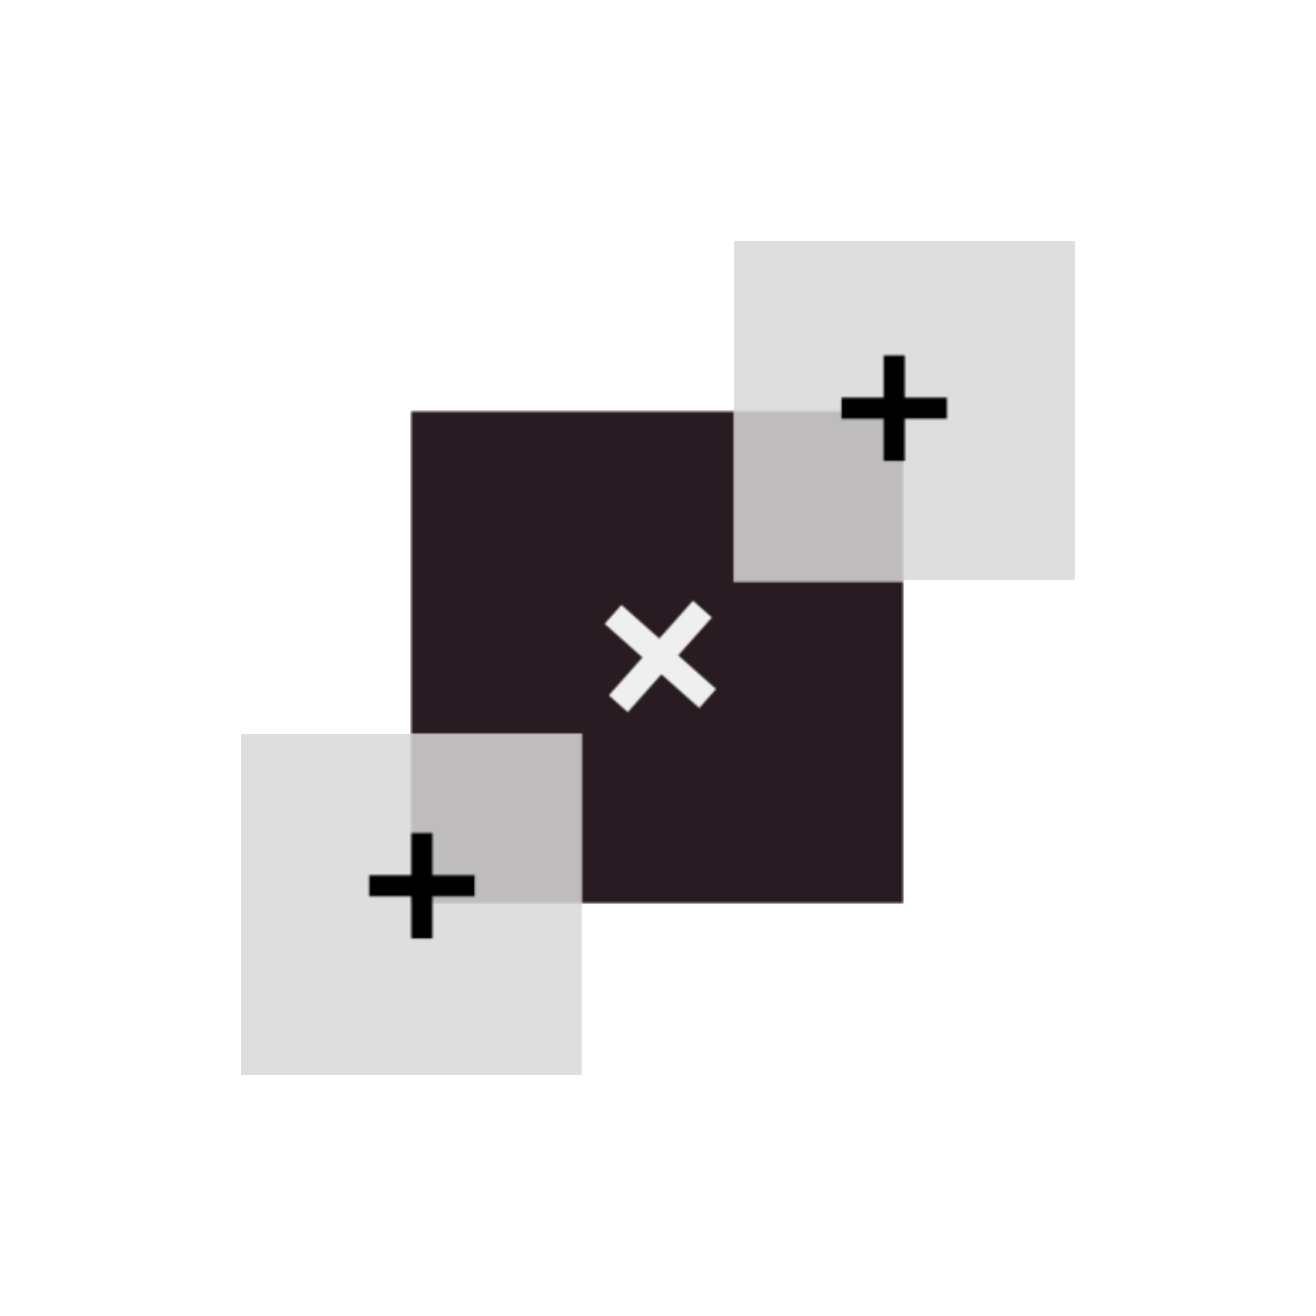
\includegraphics[width=0.9in]{logojro.png}}}
\end{picture}
\vspace{-3.5em}



\subsubsection*{Overview}

As we approach the end of this semester, it is necessary for us, STEM learners to prepare for the final graded assessments. In this case, since \joshbluebf{basic calculus} is our \joshbf{specialized subject}, we have no choice but to review since our respective outcomes of the incoming test reflects a stake of our performance in calculus. Because of this, this motivates me to create this reviewer to help you succeed in this semester since it is my core value to help each other to sustain and to promote a student-friendly and a collective community amongst us, Ateneans. 

\subsubsection*{Format of the reviewer}

The reviewer is divided into two major parts: \addubluebf{limits, derivatives and integral calculus} (that includes integration rules.) Each part will compose of 15 items and a \joshbf{Solutions} part. In most parts, when you see this ($\star$), it means the problem is a BONUS item. You are encouraged to solve it but you can disregard it.

\vspace{3mm}

For the \joshbf{Solutions}, you are encouraged to see this section after you tried answering the questions. Anyways, not all questions will not be provided by solutions but all questions will be provided by answers. In other words, there will be an answer key as well. 

\subsubsection*{Hyperlinks are provided}

Note that the article is hyperlinked. This means that you can easily navigate the whole reviewer as long as the reviewer is in PDF form. Here is an example from my \joshbf{PMO 2022 Write-ups} \footnote{If you want to check my writeups, then visit my website: \url{https://sites.google.com/addu.edu.ph/joshrobertobaob/stuff/latex-projects-personal}}

\begin{center}
  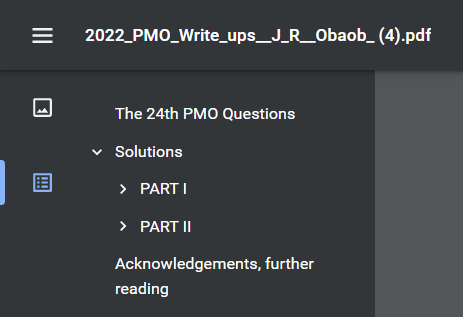
\includegraphics[width=5cm]{Pictures/2022-03-03 (1).png}
  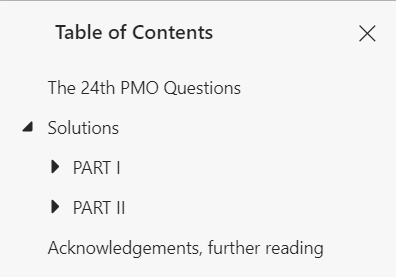
\includegraphics[width=5cm]{Pictures/2022-03-03 (3).png}
  
  {\sffamily \footnotesize (On the right, that is, if you use Google Chrome, and on the right, that is, when you use Microsoft Edge)}
\end{center}

You can find these hyperlinks at the upper left most of your screen. 

\subsubsection*{Sources}

The sources of these problems are from our formative quizzes and some are self-made. Some as well are found in my books. Here are some of my books:

\begin{itemize}
    \item \joshbf{Calculus Volume 1} by Openstax
    \item \joshbf{Pre-Calculus 7th Edition} by Larson \& Hostetler
\end{itemize}


\newpage

\section{Limits}
\subsection{Questions}
\textbf{PART I:} Choose the best answer. Figures are not drawn to scale. 

\begin{enumerate}[label=\textbf{\arabic*}.]

\item A \enspace\hrulefill.  function is \underline{a function that that composes of multiple equations.} 

\fourch{quadratic}{piecewise}{linear}{polynomial}

\end{enumerate}

For \joshbf{items 2-4}, refer to the graph of $f(x)$:

\begin{center}



\tikzset{every picture/.style={line width=0.75pt}} %set default line width to 0.75pt        

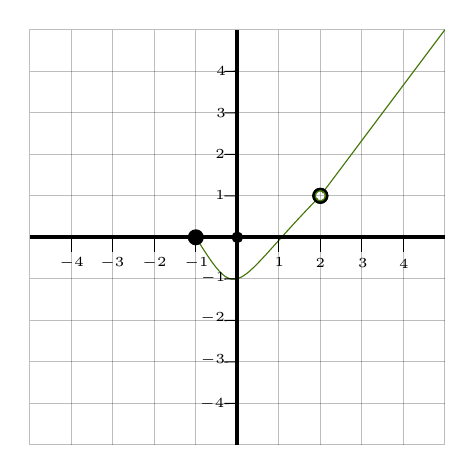
\begin{tikzpicture}[x=0.75pt,y=0.75pt,yscale=-1,xscale=1]
%uncomment if require: \path (0,341); %set diagram left start at 0, and has height of 341

%Curve Lines [id:da5407951300723142] 
\draw [color={rgb, 255:red, 65; green, 117; blue, 5 }  ,draw opacity=1 ]   (283,173) .. controls (304.14,206.91) and (300.67,196.47) .. (341.74,154.29) ;
\draw [shift={(343,153)}, rotate = 314.43] [color={rgb, 255:red, 65; green, 117; blue, 5 }  ,draw opacity=1 ][line width=0.75]      (0, 0) circle [x radius= 3.35, y radius= 3.35]   ;
%Shape: Grid [id:dp5838387796656666] 
\draw  [draw opacity=0] (203,73) -- (403,73) -- (403,273) -- (203,273) -- cycle ; \draw  [color={rgb, 255:red, 0; green, 0; blue, 0 }  ,draw opacity=0.26 ] (223,73) -- (223,273)(243,73) -- (243,273)(263,73) -- (263,273)(283,73) -- (283,273)(303,73) -- (303,273)(323,73) -- (323,273)(343,73) -- (343,273)(363,73) -- (363,273)(383,73) -- (383,273) ; \draw  [color={rgb, 255:red, 0; green, 0; blue, 0 }  ,draw opacity=0.26 ] (203,93) -- (403,93)(203,113) -- (403,113)(203,133) -- (403,133)(203,153) -- (403,153)(203,173) -- (403,173)(203,193) -- (403,193)(203,213) -- (403,213)(203,233) -- (403,233)(203,253) -- (403,253) ; \draw  [color={rgb, 255:red, 0; green, 0; blue, 0 }  ,draw opacity=0.26 ] (203,73) -- (403,73) -- (403,273) -- (203,273) -- cycle ;
%Straight Lines [id:da9374787776792131] 
\draw [color={rgb, 255:red, 0; green, 0; blue, 0 }  ,draw opacity=1 ][line width=1.5]    (303,73) -- (303,273) ;
%Straight Lines [id:da0028431777984689877] 
\draw [color={rgb, 255:red, 0; green, 0; blue, 0 }  ,draw opacity=1 ][line width=1.5]    (403,173) -- (203,173) ;
\draw [shift={(303,173)}, rotate = 180] [color={rgb, 255:red, 0; green, 0; blue, 0 }  ,draw opacity=1 ][fill={rgb, 255:red, 0; green, 0; blue, 0 }  ,fill opacity=1 ][line width=1.5]      (0, 0) circle [x radius= 1.74, y radius= 1.74]   ;
%Straight Lines [id:da9808539578299018] 
\draw    (296.73,93.07) -- (303,93) ;
%Straight Lines [id:da4624334810539217] 
\draw    (296.73,113.07) -- (303,113) ;
%Straight Lines [id:da16397790691646197] 
\draw    (296.73,133.07) -- (303,133) ;
%Straight Lines [id:da5168627321363128] 
\draw    (296.73,153.07) -- (303,153) ;
%Straight Lines [id:da11953960016498688] 
\draw    (296.73,193.07) -- (303,193) ;
%Straight Lines [id:da7881099837228092] 
\draw    (296.73,213.07) -- (303,213) ;
%Straight Lines [id:da8447820302235785] 
\draw    (296.73,233.07) -- (303,233) ;
%Straight Lines [id:da16959451889479715] 
\draw    (296.73,253.07) -- (303,253) ;
%Straight Lines [id:da10954495977950818] 
\draw    (263,173) -- (263,177.5) -- (263,180) ;
%Straight Lines [id:da13102438639757286] 
\draw    (303,193) -- (303,197.5) -- (303,200) ;
%Straight Lines [id:da12366621599687044] 
\draw    (303,193) -- (303,197.5) -- (303,200) ;
%Straight Lines [id:da3184044137957378] 
\draw    (283,173) -- (283,177.5) -- (283,180) ;
%Straight Lines [id:da8936488983430568] 
\draw    (243,173) -- (243,177.5) -- (243,180) ;
%Straight Lines [id:da36414403532700623] 
\draw    (223,173) -- (223,177.5) -- (223,180) ;
%Straight Lines [id:da9606647351010031] 
\draw    (323,173) -- (323,177.5) -- (323,180) ;
%Straight Lines [id:da44146628510397545] 
\draw    (343,173) -- (343,177.5) -- (343,180) ;
%Straight Lines [id:da03138679833262614] 
\draw    (363,173) -- (363,177.5) -- (363,180) ;
%Straight Lines [id:da4121456472303917] 
\draw    (383,173) -- (383,177.5) -- (383,180) ;
%Straight Lines [id:da38523744244596236] 
\draw [color={rgb, 255:red, 65; green, 117; blue, 5 }  ,draw opacity=1 ]   (344.01,151.66) -- (403,73) ;
\draw [shift={(343,153)}, rotate = 306.87] [color={rgb, 255:red, 65; green, 117; blue, 5 }  ,draw opacity=1 ][line width=0.75]      (0, 0) circle [x radius= 2.68, y radius= 2.68]   ;
%Straight Lines [id:da7538233855770269] 
\draw    (343,153) ;
\draw [shift={(343,153)}, rotate = 0] [color={rgb, 255:red, 0; green, 0; blue, 0 }  ][line width=0.75]      (0, 0) circle [x radius= 3.35, y radius= 3.35]   ;
%Straight Lines [id:da49183318381653396] 
\draw    (283,173) ;
\draw [shift={(283,173)}, rotate = 0] [color={rgb, 255:red, 0; green, 0; blue, 0 }  ][fill={rgb, 255:red, 0; green, 0; blue, 0 }  ][line width=0.75]      (0, 0) circle [x radius= 3.35, y radius= 3.35]   ;
%Straight Lines [id:da31406690758856426] 
\draw    (343,153) ;
\draw [shift={(343,153)}, rotate = 0] [color={rgb, 255:red, 0; green, 0; blue, 0 }  ][line width=0.75]      (0, 0) circle [x radius= 3.35, y radius= 3.35]   ;

% Text Node
\draw (294.73,152.82) node  [font=\tiny]  {$1$};
% Text Node
\draw (294.73,132.82) node  [font=\tiny]  {$2$};
% Text Node
\draw (295.23,113.07) node  [font=\tiny]  {$3$};
% Text Node
\draw (295.23,92.82) node  [font=\tiny]  {$4$};
% Text Node
\draw (291.32,192.82) node  [font=\tiny]  {$-1$};
% Text Node
\draw (291.07,211.98) node  [font=\tiny]  {$-2$};
% Text Node
\draw (291.23,232.32) node  [font=\tiny]  {$-3$};
% Text Node
\draw (290.9,253.15) node  [font=\tiny]  {$-4$};
% Text Node
\draw (283.32,185.32) node  [font=\tiny]  {$-1$};
% Text Node
\draw (263.07,185.4) node  [font=\tiny]  {$-2$};
% Text Node
\draw (242.73,185.4) node  [font=\tiny]  {$-3$};
% Text Node
\draw (223.15,185.4) node  [font=\tiny]  {$-4$};
% Text Node
\draw (323.23,185.07) node  [font=\tiny]  {$1$};
% Text Node
\draw (342.98,185.32) node  [font=\tiny]  {$2$};
% Text Node
\draw (363.48,185.57) node  [font=\tiny]  {$3$};
% Text Node
\draw (383.23,185.75) node  [font=\tiny]  {$4$};


\end{tikzpicture}
\end{center}
 
  \begin{enumerate}[resume, label=\arabic*.,font=\bfseries]
  
\item What is the first piece in the graph of $f(x)$ ?



\fourch{$x^2 - 1$; $-1 \leq x < 2 $}{$x^2 - 1$; $x < 1$}{$x^4 -1$; $-1 \geq x > 2$}{$x^2$; $x > 1$}

\item What is the second piece in the graph of $f(x)$ 

\fourch{$y=x; x>0$}{$y=x^2; x > 0$}{$y=\dfrac{4}{3}x - \dfrac{5}{3}; x < 2$}{$-\dfrac{4}{3}x - \dfrac{5}{3}; x > 2$}

\item  Which of the following functions define the graph of $f(x)$?

\begin{enumerate}
    \item[(a)] $f(x) = $\begin{cases} x^2 - 1 ;  -1 \leq x < 2 \\
    -\dfrac{4}{3}x - \dfrac{5}{3} ; x > 2\end{cases}
    
      \item[(b)] $f(x) = $\begin{cases} x^2 - 1 ;  -1 \leq x \leq 2 \\
    \dfrac{4}{3}x - \dfrac{5}{3} ; x > 2\end{cases}
    
      \item[(c)] $f(x) = $\begin{cases} x^2 - 1 ;  -1 \geq x > 2 \\
    -\dfrac{4}{3}x - \dfrac{5}{3} ; x < 2\end{cases}
    
    \item[(d)] None of the above
\end{enumerate}

\item All of the functions have a solid point at (3,1) \joshbf{EXCEPT ONE.} Which is one of the following?

\begin{enumerate}
    \item [(a)]  $c(x)$ = \begin{cases} -2x, & x<0 \\ (x-1)^2-1, & 0<x<3 \\ 1, & x=3 \\ \frac{1}{2}x-\frac{5}{2}, & x>3\end {cases} 
    
    \item [(b)] $q(x)$ = \begin{cases} (x+3)^2-2, & x<-2 \\ 1, & x=-2 \\ -x, & -2<x<1 \\ (x-1)^2-1, & x>1\end {cases}
    
    \item [(c)] $t(x)$ = \begin{cases} 2x+4, & x<-1 \\ 0, & x=-1 \\ x^2-1, & -1<x<2 \\ 7-2x, & x>2\end {cases}
    
    \item[(d)] $y(x)$ = \begin{cases} 2x+2, & x<-1 \\ 1, & x=-1 \\ -x^2+3, & -1<x<2 \\ 2x-5, & x>2\end {cases}
\end{enumerate}

\end{enumerate}

 For \joshbf{items 6-7}, refer to the figure below, showing the graph of $f(x)$:

\begin{center}
    


\tikzset{every picture/.style={line width=0.75pt}} %set default line width to 0.75pt        

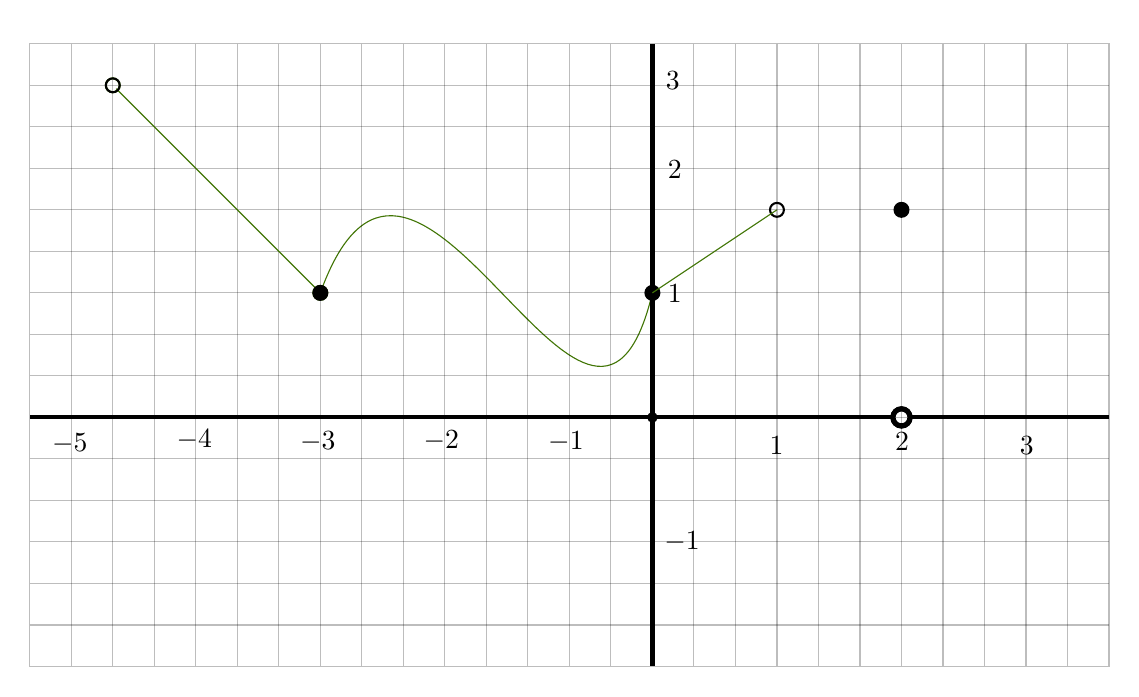
\begin{tikzpicture}[x=0.75pt,y=0.75pt,yscale=-1,xscale=1]
%uncomment if require: \path (0,431); %set diagram left start at 0, and has height of 431

%Curve Lines [id:da6246914198121776] 
\draw [color={rgb, 255:red, 65; green, 117; blue, 5 }  ,draw opacity=1 ]   (206,157) .. controls (252,29.5) and (336.22,281) .. (366,157) ;
%Shape: Grid [id:dp22593457337695644] 
\draw  [draw opacity=0] (66,37) -- (586,37) -- (586,337) -- (66,337) -- cycle ; \draw  [color={rgb, 255:red, 0; green, 0; blue, 0 }  ,draw opacity=0.26 ] (86,37) -- (86,337)(106,37) -- (106,337)(126,37) -- (126,337)(146,37) -- (146,337)(166,37) -- (166,337)(186,37) -- (186,337)(206,37) -- (206,337)(226,37) -- (226,337)(246,37) -- (246,337)(266,37) -- (266,337)(286,37) -- (286,337)(306,37) -- (306,337)(326,37) -- (326,337)(346,37) -- (346,337)(366,37) -- (366,337)(386,37) -- (386,337)(406,37) -- (406,337)(426,37) -- (426,337)(446,37) -- (446,337)(466,37) -- (466,337)(486,37) -- (486,337)(506,37) -- (506,337)(526,37) -- (526,337)(546,37) -- (546,337)(566,37) -- (566,337) ; \draw  [color={rgb, 255:red, 0; green, 0; blue, 0 }  ,draw opacity=0.26 ] (66,57) -- (586,57)(66,77) -- (586,77)(66,97) -- (586,97)(66,117) -- (586,117)(66,137) -- (586,137)(66,157) -- (586,157)(66,177) -- (586,177)(66,197) -- (586,197)(66,217) -- (586,217)(66,237) -- (586,237)(66,257) -- (586,257)(66,277) -- (586,277)(66,297) -- (586,297)(66,317) -- (586,317) ; \draw  [color={rgb, 255:red, 0; green, 0; blue, 0 }  ,draw opacity=0.26 ] (66,37) -- (586,37) -- (586,337) -- (66,337) -- cycle ;
%Straight Lines [id:da24280268773949598] 
\draw [color={rgb, 255:red, 0; green, 0; blue, 0 }  ,draw opacity=1 ][line width=1.5]    (366,37) -- (366,337) ;
%Straight Lines [id:da2502938816006557] 
\draw [color={rgb, 255:red, 0; green, 0; blue, 0 }  ,draw opacity=1 ][line width=1.5]    (482.65,217) -- (66,217) ;
\draw [shift={(486,217)}, rotate = 180] [color={rgb, 255:red, 0; green, 0; blue, 0 }  ,draw opacity=1 ][line width=1.5]      (0, 0) circle [x radius= 4.36, y radius= 4.36]   ;
%Straight Lines [id:da8905281500988929] 
\draw [color={rgb, 255:red, 65; green, 117; blue, 5 }  ,draw opacity=1 ]   (107.66,58.66) -- (206,157) ;
\draw [shift={(206,157)}, rotate = 45] [color={rgb, 255:red, 65; green, 117; blue, 5 }  ,draw opacity=1 ][fill={rgb, 255:red, 65; green, 117; blue, 5 }  ,fill opacity=1 ][line width=0.75]      (0, 0) circle [x radius= 3.35, y radius= 3.35]   ;
\draw [shift={(106,57)}, rotate = 45] [color={rgb, 255:red, 65; green, 117; blue, 5 }  ,draw opacity=1 ][line width=0.75]      (0, 0) circle [x radius= 3.35, y radius= 3.35]   ;
%Straight Lines [id:da6672457065722368] 
\draw    (206,157) ;
\draw [shift={(206,157)}, rotate = 0] [color={rgb, 255:red, 0; green, 0; blue, 0 }  ][fill={rgb, 255:red, 0; green, 0; blue, 0 }  ][line width=0.75]      (0, 0) circle [x radius= 3.35, y radius= 3.35]   ;
%Straight Lines [id:da04841084266044948] 
\draw    (106,57) ;
\draw [shift={(106,57)}, rotate = 0] [color={rgb, 255:red, 0; green, 0; blue, 0 }  ][line width=0.75]      (0, 0) circle [x radius= 3.35, y radius= 3.35]   ;
%Straight Lines [id:da7087699212759466] 
\draw    (366,217) ;
\draw [shift={(366,217)}, rotate = 0] [color={rgb, 255:red, 0; green, 0; blue, 0 }  ][fill={rgb, 255:red, 0; green, 0; blue, 0 }  ][line width=0.75]      (0, 0) circle [x radius= 2.01, y radius= 2.01]   ;
%Straight Lines [id:da8765115115166742] 
\draw    (366,157) ;
\draw [shift={(366,157)}, rotate = 0] [color={rgb, 255:red, 0; green, 0; blue, 0 }  ][fill={rgb, 255:red, 0; green, 0; blue, 0 }  ][line width=0.75]      (0, 0) circle [x radius= 3.35, y radius= 3.35]   ;
%Straight Lines [id:da7918499721558434] 
\draw    (426,117) ;
\draw [shift={(426,117)}, rotate = 0] [color={rgb, 255:red, 0; green, 0; blue, 0 }  ][line width=0.75]      (0, 0) circle [x radius= 3.35, y radius= 3.35]   ;
%Straight Lines [id:da7601033680109339] 
\draw [color={rgb, 255:red, 65; green, 117; blue, 5 }  ,draw opacity=1 ]   (366,157) -- (426,117) ;
%Straight Lines [id:da4582704557408164] 
\draw    (486,117) ;
\draw [shift={(486,117)}, rotate = 0] [color={rgb, 255:red, 0; green, 0; blue, 0 }  ][fill={rgb, 255:red, 0; green, 0; blue, 0 }  ][line width=0.75]      (0, 0) circle [x radius= 3.35, y radius= 3.35]   ;
%Straight Lines [id:da3884583011092262] 
\draw    (486,217) ;
\draw [shift={(486,217)}, rotate = 0] [color={rgb, 255:red, 0; green, 0; blue, 0 }  ][line width=0.75]      (0, 0) circle [x radius= 3.35, y radius= 3.35]   ;
%Straight Lines [id:da5064392464689422] 
\draw [color={rgb, 255:red, 0; green, 0; blue, 0 }  ,draw opacity=1 ][line width=1.5]    (586,217) -- (489.36,217) ;
\draw [shift={(486,217)}, rotate = 180] [color={rgb, 255:red, 0; green, 0; blue, 0 }  ,draw opacity=1 ][line width=1.5]      (0, 0) circle [x radius= 4.36, y radius= 4.36]   ;

% Text Node
\draw (324.32,228.82) node  [font=\normalsize]  {$-1$};
% Text Node
\draw (264.32,228.32) node  [font=\normalsize]  {$-2$};
% Text Node
\draw (204.82,228.82) node  [font=\normalsize]  {$-3$};
% Text Node
\draw (145.32,227.82) node  [font=\normalsize]  {$-4$};
% Text Node
\draw (85.32,229.82) node  [font=\normalsize]  {$-5$};
% Text Node
\draw (425.82,230.82) node  [font=\normalsize]  {$1$};
% Text Node
\draw (486.32,228.82) node  [font=\normalsize]  {$2$};
% Text Node
\draw (546.32,230.82) node  [font=\normalsize]  {$3$};
% Text Node
\draw (376.82,157.32) node  [font=\normalsize]  {$1$};
% Text Node
\draw (376.82,97.82) node  [font=\normalsize]  {$2$};
% Text Node
\draw (375.82,54.82) node  [font=\normalsize]  {$3$};
% Text Node
\draw (380.32,276.82) node  [font=\normalsize]  {$-1$};


\end{tikzpicture}
\end{center}

\begin{enumerate}[resume, label=\arabic*.,font=\bfseries]
\item Given the graph of $f(x)$, what is the value of c such that $\displaystyle \mathop {\lim }\limits_{x \rightarrow c} f(x)=f(c)$?

\fourch{$-1$}{0}{$1$}{$2$}

\item Given the graph of $f(x)$, which of the following limits exist?

\fourch{$\displaystyle \mathop {\lim }\limits_{x \rightarrow 0} f(x)$}{$\displaystyle \mathop {\lim }\limits_{x \rightarrow 1} f(x)$}{$\displaystyle \mathop {\lim }\limits_{x \rightarrow 0} f(y)$}{$\displaystyle \mathop {\lim }\limits_{x \rightarrow 1} f(y)$}

\item Suppose Josh was given a function,

\begin{center}
    $c(x) = $\begin{cases}
    (x+6)^2 - 5x + 7, & x\geq-1 \\ 37, &  x\leq0 
    \end{cases}
\end{center}

Evaluate $\lim_{x \rightarrow 0} c(x)$.

\fourch{35}{36}{37}{does not exist}

\item (Refer to the previous item) How about $\displaystyle \mathop {\lim }\limits_{x \rightarrow -1} c(x)$?

\fourch{35}{36}{37}{does not exist}

\item Suppose that the limit value of $\displaystyle \mathop {\lim }\limits_{x\rightarrow a} \dfrac{f(x)}{g(x)} =\dfrac{0}{0}$,  what does $\dfrac{0}{0}$ imply?

\begin{enumerate}
    \item[(a)] A limit exist.
    \item[(b)] The numerator needs to be factored out.
    \item[(c)] Limit does not exist.
    \item[(d)] None of the above
\end{enumerate}


\end{enumerate}


 \raggedright \textbf{PART II:} Problem-solving. 

\begin{enumerate}[resume, label=\arabic*.,font=\bfseries]
    \item Suppose there is a function $f$ such that $f(x) =1+2x-x^2$, and
    
    $$\lim_{x \rightarrow 2} {f(x)}$$
    
    \begin{enumerate}
        \item[(a)] What are the rules of limits that are being used? 
        
        \item[(b)] Evaluate the following expression.
    \end{enumerate}
    
    \item Suppose there is an expression:
    
    $$\lim_{x \rightarrow 4} \dfrac{\sqrt{x+6}+\sqrt{10}}{x-4} + 8$$
    
    \begin{enumerate}
        \item[(a)] What are the rules of limits that are being used? 
        
        \item[(b)] Evaluate the following expression.
    \end{enumerate}
    
    \item Suppose there is an expression:
    
    $$\displaystyle \mathop {\lim }\limits_{z \to 8} \frac{{2{z^2} - 17z + 8}}{{8 - z}}$$
    
    Evaluate the following expression.

    
        \item Suppose there is an expression:
    
    $$\displaystyle \mathop {\lim }\limits_{y \to 7} \frac{{{y^2} - 4y - 21}}{{3{y^2} - 17y - 28}}$$
    
     Evaluate the following expression.
    
    \item (Bonus item): 
    
    
    \begin{enumerate}
        \item[(a)] Evaluate the following limit: $$\displaystyle \mathop {\lim }\limits_{x \to \infty} \frac{7x - 8x^2 +9x^3}{{3x^2 +2x + x^3}}$$
    
    \item[(b)] Evaluate the following limit:
    $$\displaystyle \mathop {\lim }\limits_{x \to 10} [ \log(2x) + \log (x^2 +5) + \log(x^3)]$$
    \end{enumerate}
\end{enumerate}

\begin{mdframed}[style=jremmdbox, frametitle=Remarks]

\begin{enumerate}
\item[(a)] For number 15a, it is optional to answer that because it requires knowledge on one of the bonus topics of limits, which is \joshbf{infinite limits and limits at infinity}. You can watch a video from \href{https://www.youtube.com/watch?v=xvFqomOpLrs}{The Organic Chemistry Tutor.}

\item[(b)] For number 15b, it is optional as well to answer because it it requires knowledge on one of the bonus topics of limits, which is \joshbf{limits of transcendental functions}. You can watch a video from \href{https://www.youtube.com/watch?v=QGOnxeaw-q8}{May Mandigal}.
\end{enumerate}

\end{mdframed}




\newpage

\subsection{Solutions}


\subsubsection{PART I Answer Key}

\begin{enumerate}[label=\arabic*.,font=\bfseries]
\item (b)
\item (a)
\item (c)
\item (b)
\item (b)
\item (b)
\item (a)
\item (c)
\item (d)
\item (a) or (b) 
\end{enumerate}

\subsubsection{PART II Solutions} 

Before proceeding to the solutions, let us have some presiquites:

\subsubsection*{Some important presiquites}

\begin{mdframed}[style=jremmdbox, frametitle = Some important presiquites]

Given that $c$ is a real number and $\displaystyle \mathop {\lim }\limits_{x \rightarrow c}f(x)$ and $\displaystyle \mathop {\lim }\limits_{x \rightarrow c} g(x)$ both exist.

\begin{theorem}[Limit of the identity function]
$$\displaystyle \mathop {\lim }\limits_{x \rightarrow c} {x} = c$$
\end{theorem}

\begin{theorem}[Constant rule]
$$\displaystyle \mathop {\lim }\limits_{x \rightarrow c} {k} = k$$ where $k$ is a real number.
\end{theorem}

\begin{theorem}[Sum \& difference rule]
$$\displaystyle \mathop {\lim }\limits_{x \rightarrow c} {[f(x) \pm g(x)]} = \displaystyle \mathop {\lim }\limits_{x \rightarrow c} f(x) \pm \displaystyle \mathop {\lim }\limits_{x \rightarrow c} g(x)$$ 
\end{theorem}

\begin{theorem}[Product of a constant and a function] The constant $k$ can be factored outside of a
limit $$\displaystyle \mathop {\lim }\limits_{x \rightarrow c} {[k \cdot f(x)]} = k \cdot \displaystyle \mathop {\lim }\limits_{x \rightarrow c} f(x) $$ 
\end{theorem}

\begin{theorem}[Product rule] $$\displaystyle \mathop {\lim }\limits_{x \rightarrow c} {[f(x) \cdot g(x)]} = \displaystyle \mathop {\lim }\limits_{x \rightarrow c} f(x) \cdot \displaystyle \mathop {\lim }\limits_{x \rightarrow c} g(x)$$ 

\end{theorem}

\begin{theorem}[Quotient rule] $$\displaystyle \mathop {\lim }\limits_{x \rightarrow c} {\left[\dfrac{f(x)}{g(x)}\right]} = \dfrac{ \displaystyle \mathop {\lim }\limits_{x \rightarrow c} f(x)}  {\displaystyle \mathop {\lim }\limits_{x \rightarrow c} g(x)}$$ 

\end{theorem}

\begin{theorem}[Power rule] $$\displaystyle \mathop {\lim }\limits_{x \rightarrow c} {x^n} = c^n$$ where $n$ is a positive integer.

\end{theorem}
\end{mdframed}

\begin{mdframed}[style=jremmdbox, frametitle = Some important presiquites]
\begin{theorem}[Power function rule] $$\displaystyle \mathop {\lim }\limits_{x \rightarrow c} {[f(x)]^n} = [\displaystyle \mathop {\lim }\limits_{x \rightarrow c} f(x)]^n$$ where $n$ is a positive integer.

\end{theorem}

\begin{theorem}[Radical rule] $$\displaystyle \mathop {\lim }\limits_{x \rightarrow c} {\sqrt[n]{x}} = \sqrt[n]{c}$$ where $n$ is a positive integer.

\end{theorem}

\begin{theorem}[Radical function rule] $$\displaystyle \mathop {\lim }\limits_{x \rightarrow c} {\sqrt[n]{f(x)}} = \sqrt[n]{\displaystyle \mathop {\lim }\limits_{x \rightarrow c} f(x)}$$ where $n$ is a positive integer.

\end{theorem}

\begin{theorem}[Direct substitution property]

$$\displaystyle \mathop {\lim }\limits_{x \rightarrow c} f(x) = f(c)$$

\end{theorem}

\begin{theorem}[Indeterminate forms]

If $\displaystyle \mathop {\lim }\limits_{x \rightarrow c} f(x) = 0$ and $\displaystyle \mathop {\lim }\limits_{x \rightarrow c} g(x) = 0$, then $\dfrac{\displaystyle \mathop {\lim }\limits_{x \rightarrow c} f(x)}{\displaystyle \mathop {\lim }\limits_{x \rightarrow c} g(x)} = \dfrac{0}{0}$ is an indeterminate form whereas there is a common factor of $f(x)$ and $g(x).$ It is used to indicate that the limit may or may not exist and so, such form can be rewritten as an expression that can be simplified further. 

\end{theorem}
\end{mdframed}

Now, I presented some important presiquites before the solutions, let us proceed!

\subsubsection*{Solutions proper}

\begin{enumerate}[resume, label=\arabic*.,font=\bfseries]
\item Suppose there is a function $f$ such that $f(x) =1+2x-x^2$, and
    
    $$\lim_{x \rightarrow 2} {f(x)}$$
    
    \begin{enumerate}
        \item[(a)] What are the rules of limits that are being used? 
        
        \ans{Power function rule, constant rule, sum rule, product rule, difference rule.}
        
        \item[(b)] Evaluate the following expression.
        
        \ans{$\displaystyle \mathop {\lim }\limits_{x \rightarrow 2} {f(x)} = 1$}
        
        \sol 
        
        \begin{equation*}
            \begin{array}{lll}
               \implies \displaystyle \mathop {\lim }\limits_{x \rightarrow 2} {f(x)} & =  &   1 + 2x - x^2\\
                
              \implies \displaystyle \mathop {\lim }\limits_{x \rightarrow 2} {f(x)} & =  &  \displaystyle \mathop {\lim }\limits_{x \rightarrow 2} 1 + \displaystyle \mathop {\lim }\limits_{x \rightarrow 2} 2x - \displaystyle \mathop {\lim }\limits_{x \rightarrow 2} x^2 \quad (\text{by sum and difference rules})\\
              
                \implies \displaystyle \mathop {\lim }\limits_{x \rightarrow 2} {f(x)} & =  &  \displaystyle \mathop {\lim }\limits_{x \rightarrow 2} 1 + \displaystyle \mathop {\lim }\limits_{x \rightarrow 2} 2 \cdot \displaystyle \mathop {\lim }\limits_{x \rightarrow 2} x - \displaystyle \mathop {\lim }\limits_{x \rightarrow 2} x^2 \quad (\text{by product rule})\\
                
                     \implies \displaystyle \mathop {\lim }\limits_{x \rightarrow 2} {f(x)} & =  &  1 + 2\cdot2 - 4 \\
                     
                         \implies \displaystyle \mathop {\lim }\limits_{x \rightarrow 2} {f(x)} & =  &  \fbox{1} \\
            \end{array} 
        \end{equation*}
    \end{enumerate}
    
    \item Suppose there is an expression:
    
    $$\lim_{x \rightarrow 4} \dfrac{\sqrt{x+6}+\sqrt{10}}{x-4} + 8$$
    
    \begin{enumerate}
        \item[(a)] What are the rules of limits that are being used? 
        
           \ans{Constant rule, sum rule, product rule, quotient rule,  radical function rule, difference rule}
        
         
          
        \item[(b)] Evaluate the following expression.
        
        \ans{$8 - \dfrac{\sqrt{8}+\sqrt{10}}{2}$}
        
        \sol         
        \begin{equation*}
            \begin{array}{lll}
               \implies \displaystyle \mathop {\lim }\limits_{x \rightarrow 2} \dfrac{\sqrt{x+6}+\sqrt{10}}{x-4} + 8 & =  &   \displaystyle \mathop {\lim }\limits_{x \rightarrow 2}  \dfrac{\sqrt{x+6}+\sqrt{10}}{x-4} + \displaystyle \mathop {\lim }\limits_{x \rightarrow 2} 8\\
                
              
                
             \implies \displaystyle \mathop {\lim }\limits_{x \rightarrow 2} \dfrac{\sqrt{x+6}+\sqrt{10}}{x-4} + 8 & =  &   \displaystyle \mathop {\lim }\limits_{x \rightarrow 2}  \dfrac{\sqrt{x+6}+\sqrt{10}}{x-4} \cdot \dfrac{\sqrt{x+6}-\sqrt{10}}{\sqrt{x+6}-\sqrt{10}}+ 8\\
             
             
               \implies \displaystyle \mathop {\lim }\limits_{x \rightarrow 2} \dfrac{\sqrt{x+6}+\sqrt{10}}{x-4} + 8 & =  &   \displaystyle \mathop {\lim }\limits_{x \rightarrow 2} \dfrac{1}{\sqrt{x+6}-\sqrt{10}}+ 8\\
               
                 \implies \displaystyle \mathop {\lim }\limits_{x \rightarrow 2} \dfrac{\sqrt{x+6}+\sqrt{10}}{x-4} + 8 & =  &   \displaystyle \mathop {\lim }\limits_{x \rightarrow 2} \dfrac{1}{\sqrt{8}-\sqrt{10}}+ 8\\
                 
                    \implies \displaystyle \mathop {\lim }\limits_{x \rightarrow 2} \dfrac{\sqrt{x+6}+\sqrt{10}}{x-4} + 8 & =  &   \displaystyle \mathop {\lim }\limits_{x \rightarrow 2} \dfrac{1}{\sqrt{8}-\sqrt{10}} \cdot \dfrac{\sqrt{8}+\sqrt{10}}{\sqrt{8}+\sqrt{10}}+ 8\\
                    
                    \implies \displaystyle \mathop {\lim }\limits_{x \rightarrow 2} \dfrac{\sqrt{x+6}+\sqrt{10}}{x-4} + 8 & =  &   \displaystyle \mathop {\lim }\limits_{x \rightarrow 2} \dfrac{\sqrt{8}+\sqrt{10}}{-2} + 8\\
                    
                     \implies \displaystyle \mathop {\lim }\limits_{x \rightarrow 2} \dfrac{\sqrt{x+6}+\sqrt{10}}{x-4} + 8 & =  & \fbox{8 - \dfrac{\sqrt{8}+\sqrt{10}}{2}} \\
           
            \end{array} 
        \end{equation*}
    \end{enumerate}
    
    \item Suppose there is an expression:
    
    $$\displaystyle \mathop {\lim }\limits_{z \to 8} \frac{{2{z^2} - 17z + 8}}{{8 - z}}$$
    
    Evaluate the following expression.
    
    \ans{$-15$}

    \sol
    
    \begin{equation*}
        \begin{array}{lll}
          \implies \displaystyle \mathop {\lim }\limits_{z \to 8} \frac{{2{z^2} - 17z + 8}}{{8 - z}}  & = & \displaystyle \mathop {\lim }\limits_{z \to 8} \frac{(z-8)(2z - 1)}{{8 - z}}\\
             
                  \implies \displaystyle \mathop {\lim }\limits_{z \to 8} \frac{{2{z^2} - 17z + 8}}{{8 - z}}  & = & -\displaystyle \mathop {\lim }\limits_{z \to 8} (2z - 1)\\
                  
                   \implies \displaystyle \mathop {\lim }\limits_{z \to 8} \frac{{2{z^2} - 17z + 8}}{{8 - z}}  & = & \fbox{$-15$}\\
        \end{array}
    \end{equation*}
    
    
        \item Suppose there is an expression:
    
    $$\displaystyle \mathop {\lim }\limits_{y \to 7} \frac{{{y^2} - 4y - 21}}{{3{y^2} - 17y - 28}}$$
    
     Evaluate the following expression.
     
     \ans{$\frac{2}{5}$}
     
     \sol 
    
    \begin{equation*}
        \begin{array}{lll}
          \implies\displaystyle \mathop {\lim }\limits_{y \to 7} \frac{{{y^2} - 4y - 21}}{{3{y^2} - 17y - 28}}  & = & \displaystyle \mathop {\lim }\limits_{y \to 7} \frac{(y-7)(y+3)}{{(3y+4)(y-7)}}\\
             
             \implies\displaystyle \mathop {\lim }\limits_{y \to 7} \frac{{{y^2} - 4y - 21}}{{3{y^2} - 17y - 28}}  & = & \displaystyle \mathop {\lim }\limits_{y \to 7} \frac{y+3}{{3y+4}}\\
                  
             \implies\displaystyle \mathop {\lim }\limits_{y \to 7} \frac{{{y^2} - 4y - 21}}{{3{y^2} - 17y - 28}}  & = & \displaystyle \mathop {\lim }\limits_{y \to 7} \frac{(7)+3}{{3(7)+4}} = \dfrac{10}{25} = \fbox{$\dfrac{2}{5}$}\\
             
        \end{array}
    \end{equation*}
    
    \item (Bonus item): 
    
    
    \begin{enumerate}
        \item[(a)] Evaluate the following limit: $$\displaystyle \mathop {\lim }\limits_{x \to \infty} \frac{7x - 8x^2 +9x^3}{{3x^2 +2x + x^3}}$$
        
        \ans{9}
        
        \sol
        
        \begin{equation*}
            \begin{array}{lll}
                \implies \displaystyle \mathop {\lim }\limits_{x \to \infty} \frac{7x - 8x^2 +9x^3}{{3x^2 +2x + x^3}} & = & \displaystyle \mathop {\lim }\limits_{x \to \infty} \frac{9(x+2)(x+1) - (35x +11)}{(x+2)(x+1)}\\
                 
                \implies \displaystyle \mathop {\lim }\limits_{x \to \infty} \frac{7x - 8x^2 +9x^3}{{3x^2 +2x + x^3}} & = & \displaystyle \mathop {\lim }\limits_{x \to \infty} 9 - \frac{(35x +11)}{(x+2)(x+1)}\\
                
                \implies \displaystyle \mathop {\lim }\limits_{x \to \infty} \frac{7x - 8x^2 +9x^3}{{3x^2 +2x + x^3}} & = & \displaystyle \mathop {\lim }\limits_{x \to \infty} 9 - \left(\frac{59}{x+2} - \frac{24}{x+1}\right)\\
                
                \implies \displaystyle \mathop {\lim }\limits_{x \to \infty} \frac{7x - 8x^2 +9x^3}{{3x^2 +2x + x^3}} & = & \displaystyle \mathop {\lim }\limits_{x \to \infty} 9 - \left((59)\left(\frac{1}{x+2}\right) - (24)\left(\frac{1}{x+1}\right)\right) \quad (\text{by (1) \footnote{ \href{https://www.youtube.com/watch?v=QKkdYW77xNI}{partial fraction decomposition}}})\\
                
                \implies \displaystyle \mathop {\lim }\limits_{x \to \infty} \frac{7x - 8x^2 +9x^3}{{3x^2 +2x + x^3}} & = & \displaystyle \mathop {\lim }\limits_{x \to \infty} 9 - \left((59)\left(\frac{1}{x+2}\right) - (24)\left(\frac{1}{x+1}\right)\right)\quad \left(\text{Use the fact that $\displaystyle \mathop {\lim }\limits_{x \to \infty} \dfrac{1}{x} = 0$}\right)\\
                
                      \implies \displaystyle \mathop {\lim }\limits_{x \to \infty} \frac{7x - 8x^2 +9x^3}{{3x^2 +2x + x^3}} & = & \displaystyle \mathop {\lim }\limits_{x \to \infty} 9 = \fbox{9}\\
            \end{array}
        \end{equation*}
    
    \item[(b)] Evaluate the following limit:
    $$\displaystyle \mathop {\lim }\limits_{x \to 10} [ \log(2x) + \log (x^2 +5) + \log(x^3)]$$
    \end{enumerate}
    
    \ans{$5 + \log 21$}
    
    \sol
    
    \begin{equation*}
        \begin{array}{lll}
             \implies  \displaystyle \mathop {\lim }\limits_{x \to 10} [ \log(2x) + \log (x^2 +5) + \log(x^3)] &  = & \displaystyle \mathop {\lim }\limits_{x \to 10} [ \log(2x^4 \cdot (x^2+5) ]\\
             
             
                  \implies  \displaystyle \mathop {\lim }\limits_{x \to 10} [ \log(2x) + \log (x^2 +5) + \log(x^3)] &  = & \displaystyle \mathop {\lim }\limits_{x \to 10} [ \log (2x^6+10x^4) ]\\
                  
                      \implies  \displaystyle \mathop {\lim }\limits_{x \to 10} [ \log(2x) + \log (x^2 +5) + \log(x^3)] &  = & \displaystyle \mathop {\lim }\limits_{x \to 10} [ \log (2(10)^6+10^5) ]\\
                      
                      \implies  \displaystyle \mathop {\lim }\limits_{x \to 10} [ \log(2x) + \log (x^2 +5) + \log(x^3)] &  = & \displaystyle \mathop {\lim }\limits_{x \to 10} [ \log (21 \cdot 10^5) ]\\
                      
                         \implies  \displaystyle \mathop {\lim }\limits_{x \to 10} [ \log(2x) + \log (x^2 +5) + \log(x^3)] &  = & \fbox{$5 + \log 21$}\\
        \end{array}
    \end{equation*}
\end{enumerate}

\newpage

\section{Derivatives}

\subsection{Questions}

\textbf{PART I:} Choose the best answer.

\begin{enumerate}[label=\arabic*.,font=\bfseries]

\item If the slope $m$ is determined by the ratio between the difference of the $y$-values and the $x$-values, that is $\frac{y_2 - y_1}{x_2 - x_1}$, then what is the other formula for $m$ that is use in \joshbf{delta method} to find the derivative of a function?

\begin{enumerate}

\item[(a)] {$\dfrac{\Delta y}{\Delta x}$}

\item[(b)] {$\displaystyle \mathop {\lim }\limits_{x \to 0} \left(\dfrac{f(x + \Delta x) - f(x)}{\Delta x}\right)$}

\item[(c)] {$\displaystyle \mathop {\lim }\limits_{\Delta x \to 0} \left(\dfrac{f(x + \Delta x) - f(x)}{\Delta x}\right)$}

\item[(d)] {$\displaystyle \mathop {\lim }\limits_{\Delta x \to 0} \left(\dfrac{f(x) - f(x + \Delta x)}{x}\right)$}


\end{enumerate}

\item The process of getting the equation of the slope of the
tangent line is called \enspace\hrulefill. 

\fourch{differentiation}{dislocation}{integration}{operation}

\item Find the derivative of $f(x) = x^2 + 21$.

\fourch{$2x + 21$}{21}{$2x^2$}{$2x$}

\item Find the derivative of $x^3 - 4x^2 + 2$.

\fourch{0}{$3x^3 - 8x^2$}{$3x^2 - 8$}{$3x^2 - 8x$}

\item If $A(x) = (x+5)^2$, what is the value of $\ddx (A(x))$?

\fourch{$5$}{$x+5$}{$2x + 10$}{$2x + 11$}

\item What is the slope of the tangent line of $x^4 + 4x^3 + 8x^2 + 6x + 7$ at $x=1$?

\fourch{$25$}{$26$}{$38$}{$39$}

\item I solved for the derivative of $f(x) = 9x^2 - 4$ and then, my answer is wrong because my answer is $\dydx = 18x^2.$ What should be the correct answer?

\fourch{$18x$}{$9x$}{$-4$}{$-5$}

\item Suppose Cayla is asked to find the equation of the tangent line of the function $f(x) = (x-2)^4 + 5$ at $x=4$. What is the equation of the line?

\begin{enumerate}
    \item[(a)] $y=32x-107$
    \item[(b)] $y=-32x-107$
    \item[(c)] $y=32x-109$
    \item[(d)] $y=-32x-109$




\end{enumerate}
\item Read the following theorem: 

\begin{thmboxed} 

Suppose there exist functions $f(x)$ and $g(x)$. The product of these functions can be denoted as $h(x)$. The derivative of $h(x)$ is $$\ddx h(x) = \ddx f(x) \cdot g(x) + \ddx g(x) \cdot f(x).$$

\end{thmboxed}

From the given information above, what is the differentiation rule being used?

\fourch{product rule}{sum rule}{quotient rule}{difference rule}

\newpage

\item Henry is a mathematics professor at the AdDU Math Department, he discussed with his class about this following differentiation rule:

\begin{thmboxed}
The derivative of $\dfrac{f(x)}{g(x)}$ is $$\dydx = \dfrac{f'(x)g(x) - g'(x)f(x)}{\left(g(x)\right)^2}$$
\end{thmboxed}

As you can see, he discussed about the \joshbf{quotient rule} but there is a condition that was not mentioned. What is this condition for the rule to be satisfied?

\fourch{$g(x) \neq 0$}{$g(x) \geq 0$}{$g(x) = 0$}{$g(x) \leq 0$}


\end{enumerate}

\raggedright \textbf{PART II:} Problem-solving. Find the derivatives of the given expressions with full solutions and try to mention the differentiation rules being used.

\begin{enumerate}[resume, label=\arabic*.,font=\bfseries]

\item Find the derivative of $2\cos (3x^2 + 4x + 2)$.

\item Find the equation of the tangent line of the function $k(x) = 4x^4 + 3x^3 +2x^2 + x + 2022$ at $x=2022.$


\item Find the derivative of the following expression: $$8\cbrt{x^2} - \dfrac{8}{\cbrt{x^2}}.$$

\item Refer to the previous item, find the equation of its tangent line at $(20, 22)$.

\item (Bonus item) Suppose there exists a function $f(x)$ such that $f(x) = \sin (\cos (\sin x))$. Find the following:

\begin{enumerate}
    \item[(a)] the derivative, and its;
    \item[(b)] equation of the line at $x=2$
\end{enumerate}

\end{enumerate}


\newpage

\subsection{Solutions}


\subsubsection{PART I Answer Key}

\begin{enumerate}[label=\arabic*.,font=\bfseries]
\item (c)
\item (a)
\item (d)
\item (d)
\item (c)
\item (c)
\item (b)
\item (a)
\item (a)
\item (a)  
\end{enumerate}

\subsubsection{PART II Solutions}  Problem-solving. Find the derivative of the given expressions with full solutions and try to mention the differentiation rules being used.

\begin{enumerate}[resume, label=\arabic*.,font=\bfseries]

\item Find the derivative of $2\cos (3x^2 + 4x + 2)$.

\ans{$-(6x +4) \cdot \left(2\sin(3x^2 +4x +2)\right)$}

\sol 

Note that the derivative of $\cos x$ is $-\sin x$ and note as well that by chain rule, $\ddx \cos x = -\sin x \cdot \ddx x$. Using these facts, we get that the derivative of the expression can be like this:

\begin{equation*}
    \begin{array}{lll}
         \implies \dfrac{d}{dx} 2\cos (3x^2 + 4x + 2) & = &  -2\sin (3x^2 + 4x + 2) \cdot  \dfrac{d(3x^2 + 4x + 2)}{dx} \\
         
         \\
         
         \implies \dfrac{d}{dx} 2\cos (3x^2 + 4x + 2) & = &  -2\sin (3x^2 + 4x + 2) \cdot (6x +4) \\
         
         \\
         
           \implies \dfrac{d}{dx} 2\cos (3x^2 + 4x + 2) & = &  -(6x +4) \cdot 2\sin (3x^2 + 4x + 2) \\
         
    \end{array}
\end{equation*}

\item Find the equation of the tangent line of the function $k(x) = 4x^4 + 3x^3 +2x^2 + x + 2022$ at $x=2.$

\ans{$y = 245x + 1630$}

\sol

First, let us evaluate $k(2)$ to find the output of it. And we get that $k(2) = 2120$. Hence, we get an ordered pair of $(2, 2120).$ Next, let us find its derivative, and we have $$16x^3 + 27x^2 + 4x + 1.$$ It is important to find the derivative because this is the slope $m$ of the tangent line of $k(x).$ Substituting $x=2$ in the derivative, we have $m=245$.

\vspace{2mm}

Now, let us find the equation of the line and we will use the point-slope equation: $$y-y_1 = m(x-x_1)$$ where $m$ is the slope and $(x_1, y_1)$ is an ordered pair in the line. Since $(2, 2120)$ is our ordered pair and $m = 245$, then we have: $$y - 2120 = 245(x-2) \Leftrightarrow y = 245x + 1630$$ and that is our equation for our tangent line!


\item Find the derivative of the following expression: $$8\cbrt{x^2} - \dfrac{8}{\cbrt{x^2}}.$$

\ans{$\dfrac{16}{3}\left(\dfrac{1}{\cbrt{x}} + \dfrac{1}{\cbrt{x^4}}\right)$}

\sol Rewrite the equation into $8x^{2/3} - 8x^{-2/3}.$ Finding its derivative, we have: $$\implies \dfrac{d\left(8x^{2/3} - 8x^{-2/3}\right)}{dx} = \dfrac{2}{3}\left(8x^{-1/3}\right) - \left(-\dfrac{2}{3}\right)\left(8x^{-4/3}\right) \Leftrightarrow \dfrac{2(8)}{3}\left(\dfrac{1}{\cbrt{x}} + \dfrac{1}{\cbrt{x^4}}\right) \Leftrightarrow \dfrac{16}{3}\left(\dfrac{1}{\cbrt{x}} + \dfrac{1}{\cbrt{x^4}}\right)$$


\item[\textbf{14 - 15.}] (Bonus item) Suppose there exists a function $f(x)$ such that $f(x) = \sin (\cos (\sin x))$. Find the following:

\begin{enumerate}
    \item[(a)] the derivative, and its;
    
    \ans{$\cos(\cos (\sin x)) \cdot \left(-\sin(\sin x) \cdot (\cos x)\right)$}
    
    \sol The expression is quite tedious. So, we will let $a = \cos (\sin x)$. This implies that $f(x) = \sin a$. To find the derivative of $f(x)$, by chain rule and trigonometric diffrentiation, we have: $$\implies \dfrac{d}{dx} (\sin a) = \cos (a) \cdot \dfrac{d}{dx} (a) .$$ Since $a = \cos(\sin x)$, then the expression can be transformed like this:  $$ \qquad \qquad \qquad \implies \cos(\cos (\sin x)) \cdot \dfrac{d}{dx}(\cos (\sin x)) \qquad \qquad\qquad \qquad (1)$$
    
 
    
    Now, let us focus on $\dfrac{d}{dx} (\cos (\sin x))$. Evaluating the expression gives us the following: $$\implies -\sin(\sin x) \cdot (\cos x)$$ This is true because $\dydx = \ddx(\cos (\sin x)) \cdot \ddx(\sin x) $. Substituting back it in (1), we have found the derivative of $f(x)$, and that is: $$\implies \dfrac{d(f(x))}{dx} = \cos(\cos (\sin x)) \cdot \left(-\sin(\sin x) \cdot (\cos x)\right)$$
    
    
    \item[(b)] equation of the line at $x=0$
    
    \ans{$y = \sin 1$.}
    
    \sol Since our slope $m$ is the derivative of $f(x)$ and $x=0$, then our slope must be $f'(0)$ and it is equal to 0. Recall the point-slope form, $$y-y_1 = m(x-x_1)$$ Finding $(x_1, y_1) = (0, f(0))$, we have $(0,\sin 1)$. Hence, the equation of the line is \fbox{$y = \sin 1$.}
\end{enumerate}

\end{enumerate}

\newpage

\section{Integral calculus}

\subsection{Questions}

\textbf{PART I:} Choose the best answer.

\begin{enumerate}[label=\arabic*.,font=\bfseries]

\item If the process of finding the slope of the equation is \textbf{differentiation} then what is its reverse process?

\fourch{differentiation}{anti-differentiation}{simplification}{none of the above}

\item The expression $\mathlarger{\int c(x)}$ is also called...

\fourch{integration}{definite integral}{integrand}{indefinite integral}

\item I was asked to find the anti-derivative of $x^3 + 1$, then I wrote $\displaystyle{\int (x^3 + 1) dx} = 3x^2 + 2x$. Unfortunately, it is the wrong answer. What makes it a wrong answer?

\begin{enumerate}
    \item[(a)] Nothing at all. 
    \item[(b)] The correct answer should be $3x^2 + 2 + C$ where $C$ is any constant.
    \item[(c)] The correct answer should be $x^4 + x + C$ where $C$ is any constant.
    \item[(d)] The correct answer should be $\dfrac{x^4}{4} + x + C$ where $C$ is any constant.
\end{enumerate}

\item If the derivative of $f(x)$ is $-\cos x$, then what is $f(x)$?

\fourch{$f(x) = \csc x$}{$f(x) = -\csc x$}{$f(x) = -\sin x$}{$f(x) = \sin x$}

\item Find the anti-derivative of $x^4 + x^3 + x^2 + x + 1.$

\begin{enumerate}
    \item[(a)] $\dfrac{x^5}{5}+ \dfrac{x^4}{4}+\dfrac{x^3}{3}+\dfrac{x^2}{2}+x + 1$
    
      \item[(b)] $\dfrac{x^5}{5}+ \dfrac{x^4}{4}+\dfrac{x^3}{3}+\dfrac{x^2}{2}+x + C$
      
      \item[(c)] $4x^3 + 3x^2 + 2x + 1$
      
      \item[(d)] $4x^3 + 3x^2 + 2x + C$
\end{enumerate}

\item Find the anti-derivative of $\displaystyle{ e^{x}} $.

\fourch{$e^x$}{$e^x + C$}{$\ln x $}{$\ln x + C$}

\item What is the anti-derivative of $\dfrac{x}{x^2 + 4}$?

\fourch{$\displaystyle{\ln (x^2 +4)}$}{$\displaystyle{\frac{1}{2} \ln (x^2 +4)}$}{$\displaystyle{\frac{1}{3} \ln (x^2 +4)}$}{$\displaystyle{\frac{1}{4} \ln (x^2 +4)}$}

\item Evaluate the following: $\displaystyle{\int x \cdot 2^{x^2} dx}$.

\fourch{$\displaystyle{\frac{2^{x^2}}{2\log2} + C}$}{$\displaystyle{\frac{2^{x^2}}{2\ln2} + C}$}{$\displaystyle{\frac{2^{x^2}}{2\ln2}}$}{$\displaystyle{\frac{2^{x^2}}{2\ln20} + C}$}

\item Evaluate the following: $\displaystyle{\int (3x+ 2)(\cbrt{x} - 3) dx}$.

\begin{enumerate}
    \item[(a)]$\dfrac{9x^7}{7} + \dfrac{9x^2}{2} + \dfrac{3}{2}x^4 - 6x + C$
    \item[(b)]$\dfrac{9x^7}{7} + \dfrac{9x^2}{2} + \dfrac{3}{2}x^4 - 6x - 6$
    \item[(c)]$\dfrac{9x^{7/3}}{7} + \dfrac{9x^2}{2} + \dfrac{3}{2}x^4 - 6x - 6$
    \item[(d)]$\dfrac{9x^{7/3}}{7} + \dfrac{9x^2}{2} + \dfrac{3}{2}x^{4/3} - 6x + C$
\end{enumerate}

\item Read the following theorem:

\begin{mdframed}[style=jradduemmdbox, frametitle= \textbf{Theorem 3.1.} (Trigonometric Antiderivatives)] For all real numbers $x$, the anti-derivative of $\cot x$ is $$\int (\cot x) dx =  \ln |\cos x| + 2C$$

\end{mdframed}

Notice the theorem has an error because the anti-derivative of $\cot x$ being shown is not correct. What should be anti-derivative of it?

\fourch{$\log |\cos x| + 2C$}{$\ln |\sin x| + 2C$}{$\log |\sin x| + C$}{$\ln |\sin x| + C$}

\end{enumerate}

\raggedright \textbf{PART II:} Problem-solving. Find the anti-derivatives of the given expressions with full solutions and try to mention the differentiation rules being used.

\begin{enumerate}[resume, label=\arabic*.,font=\bfseries]

\item \textsf{\href{https://iymc.info/docs/problems/2020/Final-Exam-2020.pdf}{(IYMC Final Exam 2020 Q18).}}  Find the correct $f(x)$ such that this equation holds true: $$\ddx f(x) = \dfrac{x}{1+x^2}$$


\item Evaluate the following: $$\int (\cos^3 x \cdot \sin x) \hspace{1mm} dx $$

\item Find the correct $f(x)$ such that $$\ddx f(x) =x-1+4\sin(2x).$$

\item \textsf{\href{http://web.mit.edu/abhinavk/www/integrationbee/qual2012.pdf}{(2012 MIT Integration Bee Qualifying Test Q20; Altered ).}} Evaluate the following: $$\int \dfrac{4x^3}{x^4 +4} \hspace{1mm} dx$$. 

\item \textsf{\href{https://math.mit.edu/~sswatson/pdfs/qualifying_round_2013.pdf}{(2013 MIT Integration Bee Qualifying Test Q13 $\star$).}} Evaluate the following: $$\int \tan^2 x \hspace{1mm} dx$$

\end{enumerate}

\newpage

\subsection{Solutions}


\subsubsection{PART I Answer Key}

\begin{enumerate}[label=\arabic*.,font=\bfseries]
\item (b)
\item (d)
\item (d)
\item (c)
\item (b)
\item (b)
\item (b)
\item (b)
\item (d)
\item (d)
\end{enumerate}

\subsubsection{PART II Solutions} 


\raggedright \textbf{PART II:} Problem-solving. Find the anti-derivatives of the given expressions with full solutions and try to mention the differentiation rules being used.

\begin{enumerate}[resume, label=\arabic*.,font=\bfseries]

\item \textsf{\href{https://iymc.info/docs/problems/2020/Final-Exam-2020.pdf}{(IYMC Final Exam 2020 Q18).}}  Find the correct $f(x)$ such that this equation holds true: $$\ddx f(x) = \dfrac{x}{1+x^2}$$

\ans{$\dfrac{1}{2}\ln(1 + x^2) + C$}

\sol In this problem, we are asked to find the anti-derivative of $\dfrac{x}{1 + x^2}$, that is, $$\int \dfrac{x}{1+x^2} \hspace{1mm} dx.$$ By $u$-substitution, let $u=1+x^2$, implying $du = 2x \hspace{1mm} dx.$ Since $x \neq du$ then we shall do the indirect $u$-substitution $$\implies \int \dfrac{x}{1+x^2} \hspace{1mm} dx \Longleftrightarrow \int \dfrac{{x}}{u}  \left(\dfrac{du}{2x}\right) \Longleftrightarrow \int \dfrac{\bcancel{x}}{u}  \left(\dfrac{du}{2 \cdot \bcancel{x}}\right) = \dfrac{1}{2}\int \dfrac{1}{u} \hspace{2mm} du$$. By theorem, $\displaystyle{\int \dfrac{1}{y} \hspace{1mm} dy = \ln y}$ for some $y$. Hence $\displaystyle{\dfrac{1}{2} \int \dfrac{1}{u} \hspace{1mm} du = \dfrac{1}{2} \ln u + C}$. Substituting back $u$ to $1 + x^2$, we have \fbox{$\dfrac{1}{2}\ln (1+x^2) + C$} as our final answer.


\item Evaluate the following: $$\int (\cos^3 x \cdot \sin x) \hspace{1mm} dx $$

\ans{$-\dfrac{\cos^4 x}{4} + C$}

\sol By $u$-substitution, $cos x = u$ and $du = -\sin x \hspace{1mm} dx$. But since we cannot find $du$ within the integral and $x \neq du$, then we can do the indirect $u$-substitution: 
$$ \implies \int (\cos^3 x \cdot \sin x) \hspace{1mm} dx \Longleftrightarrow \int (u^3  \cdot \bcancel{\sin x}) \hspace{1mm} \left(\dfrac{du}{-\bcancel{\sin x}}\right) = - \int u^3 du $$. By general power rule, we have $\displaystyle{\int u^3 du} -\dfrac{u^{3+1}}{3+1} + C = -\dfrac{u^4}{4} + C$. Substituting back, we have \fbox{$-\dfrac{\cos^4 x}{4} + C.$}


\item Find the correct $f(x)$ such that $$\ddx f(x) =x-1+4\sin(2x).$$

\ans{$\dfrac{x^2}{2}- x - 2\cos 2x + C$}

\sol The following problem can be rewritten into $$\int x-1+4\sin(2x) \hspace{1mm} dx \Longleftrightarrow \int x \hspace{1mm} dx - \int dx + 4\int \sin(2x) \hspace{1mm} dx $$.

Then by general power and constant rules, $$\int x \hspace{1mm} dx - \int dx + 4\int \sin(2x) \hspace{1mm} dx = \dfrac{x^{1+1}}{1+1}- \dfrac{x^{0+1}}{0+1} +  4\int \sin(2x) + C$$ To evaluate $\displaystyle{4\int \sin(2x)}$, let use the $u$-substitution. Let $u=2x$, implying $du=2 \hspace{1mm} dx$, and then, we have: $$4\int \sin(2x) \hspace{1mm} dx \implies 4\int \sin u \left(\dfrac{du}{2}\right) = \dfrac{1}{2} (4)\int \sin u \hspace{1mm} du = -2\cos u + C  $$ This implies that  $2\displaystyle{\int \sin u \hspace{1mm} du = -2\cos (2x) + C  }$.

\vspace{2mm}

Going back to our main problem, our final answer must be \fbox{$\displaystyle{\dfrac{x^2}{2}- x - 2\cos 2x + C}$}



\item \textsf{\href{http://web.mit.edu/abhinavk/www/integrationbee/qual2012.pdf}{(2012 MIT Integration Bee Qualifying Test Q20; Altered ).}} Evaluate the following: $$\int \dfrac{4x^3}{x^4 +4} \hspace{1mm} dx$$

\vspace{-3mm}

\ans{${\int \frac{4x^3}{x^4 + 4} \hspace{1mm} dx = \ln (x^4 + 4) + C}$}

\soln1 At first glance, we are motivatd to use $u$-substitution. Let $x^4 + 4 = u$ and $du = 4x^3 dx.$ Observing the expression, we see that we can \textbf{directly} do $u$- substutiton. Because of this, we are motivated this theorem:


\newpage

\begin{mdframed}[style=jradduemmdbox, frametitle= \textbf{Theorem 3.2.}]
For all positive real numbers $w$, there exists a function $h(w)$ such that $$\int \dfrac{h'(w)}{h(w)} \hspace{1mm} dw = \ln \left(h(w)\right) + C$$ for some constant $C.$
\end{mdframed}

We can say that $h(w) = x^4 + 4$ an $h'(w) = 4x^3$. Therefore, \fbox{$\mathlarger{\int \dfrac{4x^3}{x^4 + 4} \hspace{1mm} dx= \ln (x^4 + 4) + C}$}

\soln2 Given from \joshbf{Solution 1} that by $u$-substitution, $u = x^4 + 4$ and $du = 4x^3 dx$ and for this second solution, you can do the indirect type of such substitution. So, we have: $$\implies \int \dfrac{{4x^3}}{x^4 + 4} \hspace{1mm} dx = \int \dfrac{\cancel{4x^3}}{u} \left(\dfrac{du}{\cancel{4x^3}}\right) = \int \dfrac{1}{u} \hspace{1mm} du = \ln u + C =  \ln(x^4 + 4) + C  $$ Jence, we got a same result. 

\item \textsf{\href{https://math.mit.edu/~sswatson/pdfs/qualifying_round_2013.pdf}{(2013 MIT Integration Bee Qualifying Test Q13 $\star$).}} Evaluate the following: $$\int \tan^2 x \hspace{1mm} dx $$



\ans{$\tan x - x + C.$}

\sol Note that $\tan^2 x = \dfrac{\sin^2 x}{\cos^2 x}$, implying that: $$\implies \int \tan^2 x \hspace{1mm} dx = \int \dfrac{\sin^2 x}{\cos^2 x} \hspace{1mm} dx $$. We will rewrite $\sin^2 x$ in terms of $\cos^2 x$. Recall that $\sin^2 x + \cos^2 x = 1 \Leftrightarrow \sin^2 x = 1- \cos^2 x.$ This implies that $$\implies \int \dfrac{\sin^2 x}{\cos^2 x} \hspace{1mm} dx = \int \dfrac{1- \cos^2 x}{\cos^2 x} \hspace{1mm} dx = \int  \dfrac{1}{\cos^2 x} \hspace{1mm} dx -  \int  \dfrac{\cos^2 x}{\cos^2 x} \hspace{1mm} dx = \int  \dfrac{1}{\cos^2 x} \hspace{1mm} dx -  \int dx  $$ Now we are reaching this point. Note that $\displaystyle{\int \dfrac{1}{\cos^2 y} \hspace{1mm} dy = \tan y + C}$ for some real number $y.$ Because of this, we have: $$\implies \tan x - \int dx + C = \tan x - \dfrac{x^{(0+1)}}{0+1} +C = \tan x - x + C$$. Hence, our final answer is \fbox{$\tan x - x + C.$}
\end{enumerate}

\begin{mdframed}
\begin{rem}
Solving this problem requires knowledge on trigonometric identities. You are not required to solve this problem. 
\end{rem}

\begin{rem}
The \joshbluebf{MIT Integration Bee Qualifying Test} is a yearly integral calculus competition pioneered in 1981 by Andy Bernoff, an applied mathematics student at the Massachusetts Institute of Technology (MIT).
\end{rem}
\end{mdframed}



\section{Closing remarks}

The reviewer is only for all STEM students of \joshbluebf{Ateneo De Davao University Senior High School}. Any replications and online publications outside the institute without my knowledge is strictly prohibited. The following reviewer is powered by LaTeX.  you see any typos, corrections, and should you have any inquiries, free to contact me at \mailto{jrdobaob@addu.edu.ph.}

\subsection*{Edition log}
 
 This section will help you to track the editions of this reviewers. That is why, expect many revisions from this article.
 
 \begin{center}
 
\begin{tabular}{|p{4cm}|p{4cm}|p{6cm}|}
    \hline
    
  {\centering \joshbf{Time}} & \joshbf{Releasing Date} & \joshbluebf{Notes about the edition}\\
  
    \hline
    
    4:50PM & March 28, 2022 &
This is the first version. Official release\\
    \hline
    
    11:22PM & March 28, 2022 &
Typo fixing. Adding \joshbf{Solution 2} to Integrals Item 14. \\
    \hline 
  
\end{tabular}
\end{center}


\vspace{12cm}

  \begin{center}

\includegraphics[width=3.5in]{JOSH ROBERT OBAOB (2).png}
\end{center}





















%\emph{I would like to thank Sir Reil Benedict Obinque, our PMO coordinator in Ateneo De Davao University for giving me a green light to make a write-ups about yesterday's test .}
\end{document}
